\documentclass[10pt]{beamer}
\usetheme{Madrid}
\usepackage[utf8]{inputenc}
\usepackage[russian]{babel}
\usepackage[OT1]{fontenc}
\usepackage{hyperref}
\usepackage{amsmath}
\usepackage{amsfonts}
\usepackage{amssymb}
\usepackage{graphicx}
\usepackage[ruled, vlined]{algorithm2e}
\author{Мальковский Н.~В.}
\title[Градиентный спуск]{Градиентный спуск}
%\setbeamercovered{transparent} 
\setbeamertemplate{navigation symbols}{} 
%\logo{} 
\institute[СПбAУ]{Санкт-Петербургский академический университет}
\date{} 
\usecolortheme{beaver}
%\subject{} 

\DeclareMathOperator{\argmin}{argmin}
\DeclareMathOperator{\interior}{Int}

\newtheorem{theorem_ru}{Теорема}[]
\newtheorem{lemma_ru}{Лемма}[]
\newtheorem{corollary_ru}{Следствие}[]

\graphicspath{{image/}}
\newcommand{\Ima}{\text{Im}}
\newcounter{remarknumber}[framenumber]
\newcommand{\remark}{\stepcounter{remarknumber}\textit{Замечание}~\arabic{remarknumber}}


\begin{document}

\begin{frame}
\titlepage
\centering
\includegraphics[width=.23\textwidth]{logo.png}
\end{frame}

%\begin{frame}
%\tableofcontents
%\end{frame}

\begin{frame}{Общая идея градиентного спуска}
\begin{equation}\label{general_problem}
\begin{array}{ll}
\mbox{минимизировать } & f(x),~x\in \mathcal{D}\subset\mathbb{R}^n.
\end{array}
\end{equation}
Условия стационарности: если $x^*\in \interior\mathcal{D}$ -- точка минимума $f$ на $\mathcal{D}$, $f$ дифференцируема в $x^*$, то 
$$
\nabla f(x^*)=0_n.
$$
\pause
Пусть $x_0\in \interior\mathcal{D}$. Можно ли понять, где находится точка минимума по $\nabla f(x_0)$?\\
\pause
Если немного сдвинуться из $x_0$ в направлении $h$, то получаем
$$
f(x_0+th)=f(x_0)+\nabla f(x_0)^Th+o(t).
$$
Таким образом, локально выгоднее всего двигаться в направлении $h=-\nabla f(x_0)$.\\
\end{frame}

\begin{frame}{Общая идея градиентного спуска}
Оказывается, при некоторых предположениях на $f$ и $0<\alpha_k\in \mathbb{R}$  последовательность 
\begin{equation}\label{gradient_descent}
x_{k+1}=x_k-\alpha_k\nabla f(x_k)
\end{equation}
сходится к точке минимума $f$.\\
\pause
Генерирование последовательности $x_k$ по правилу \eqref{gradient_descent} принято называть \textit{градиентным спуском}. Величину $\alpha_k$ принято называть \textit{размером шага} на $k$-ой итерации.\\
\pause
\vspace{1em}
В многих случаях легче измерить $\nabla f$ в нескольких точках, чтобы получить приближенное значение точки минимума нежели решать систему уравнений $\nabla f(x)=0_n$.
\end{frame}

\begin{frame}{Основные способы выбора шага}
Наиболее распространенными способами выбора последовательности $\alpha_k$ в градиентном спуске являются следующие три:
\begin{itemize}
\item Заранее выбранная последовательность, например $\alpha_k\equiv \alpha>0$ или $\alpha_k=\frac{\alpha}{n^c}$.
\item Точный минимум по направлению: 
$$
\alpha_k=\argmin_\alpha f(x_k-\alpha\nabla f(x_k)).
$$
\item Аппроксимированный минимум по направлению, $\alpha_k$ вычисляется следующим образом: пусть $\gamma\in(0, 1/2)$, 
$\beta\in (0, 1)$ -- некоторые константы
\begin{function}[H]
 \caption{Backtracking line search($f$, $x_k$, $\gamma$, $\beta$)}
 $\alpha_k\leftarrow 1$\;
 \While{$f(x_k-\alpha_k\nabla f(x_k))>f(x_k)-\gamma\alpha_k||\nabla f(x_k)||^2$}{
 	$\alpha_k\leftarrow \beta\alpha_k$\; 
 }
 return $\alpha_k$\;
\end{function}

\end{itemize}


\end{frame}

\begin{frame}{Пример: градиентный спуск для квадратичной функции}
\only<1-1>{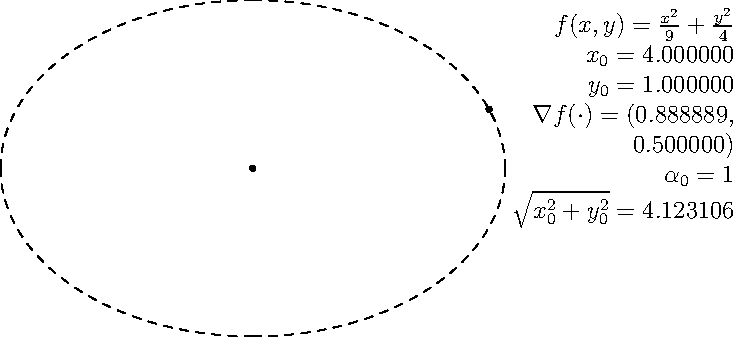
\includegraphics[width=\textwidth]{ellipse_grad/ellipse_grad0}}%
\only<2-2>{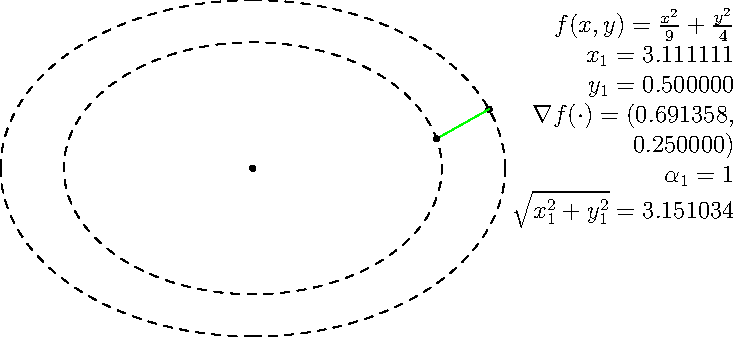
\includegraphics[width=\textwidth]{ellipse_grad/ellipse_grad1}}%
\only<3-3>{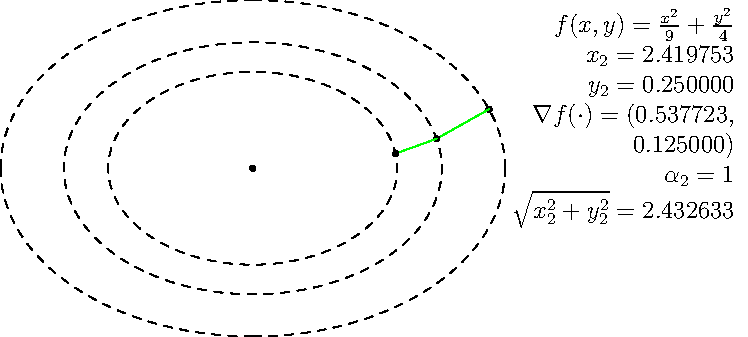
\includegraphics[width=\textwidth]{ellipse_grad/ellipse_grad2}}%
\only<4-4>{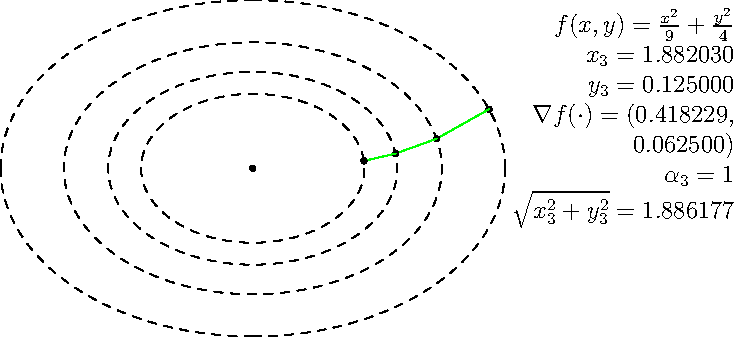
\includegraphics[width=\textwidth]{ellipse_grad/ellipse_grad3}}%
\only<5-5>{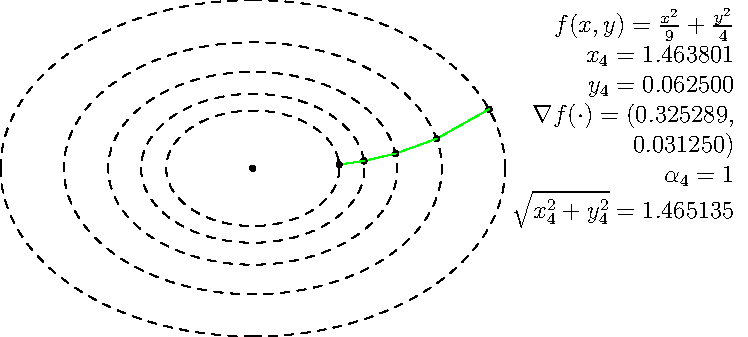
\includegraphics[width=\textwidth]{ellipse_grad/ellipse_grad4}}%
\only<6-6>{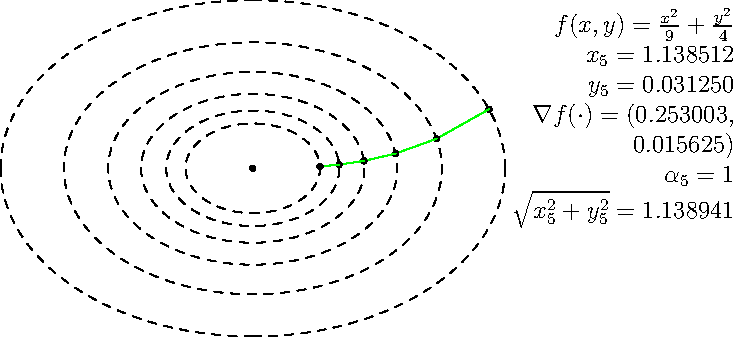
\includegraphics[width=\textwidth]{ellipse_grad/ellipse_grad5}}%
\only<7-7>{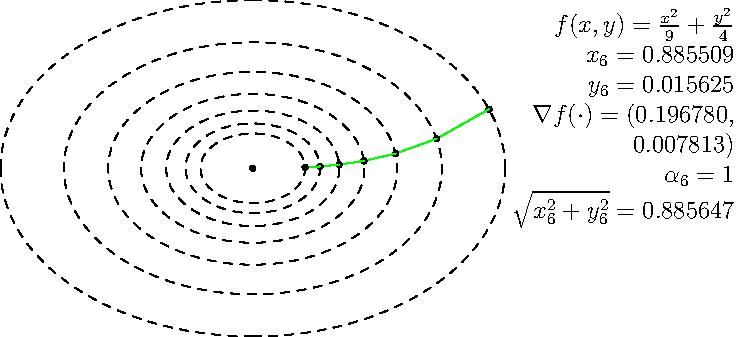
\includegraphics[width=\textwidth]{ellipse_grad/ellipse_grad6}}%
\only<8-8>{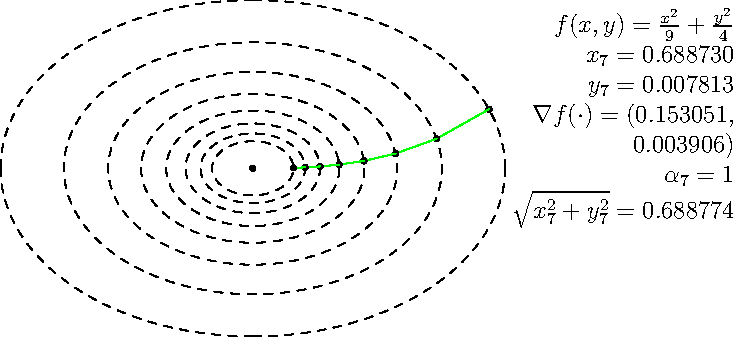
\includegraphics[width=\textwidth]{ellipse_grad/ellipse_grad7}}%
\only<9-9>{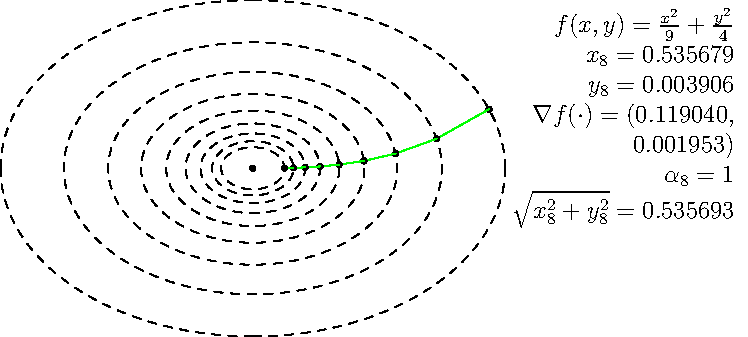
\includegraphics[width=\textwidth]{ellipse_grad/ellipse_grad8}}%
\only<10-10>{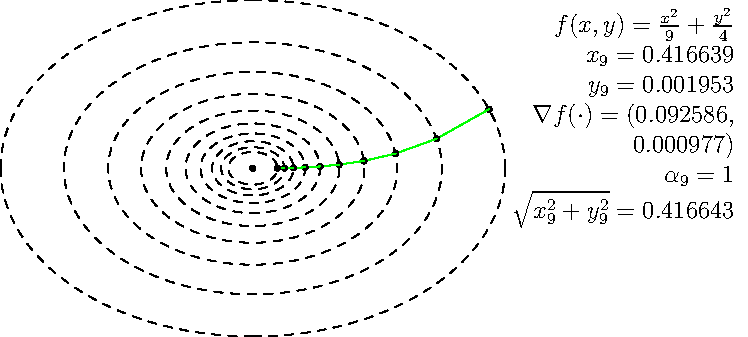
\includegraphics[width=\textwidth]{ellipse_grad/ellipse_grad9}}%
\end{frame}

\begin{frame}{Пример: градиентный спуск для квадратичной функции}
\only<1-1>{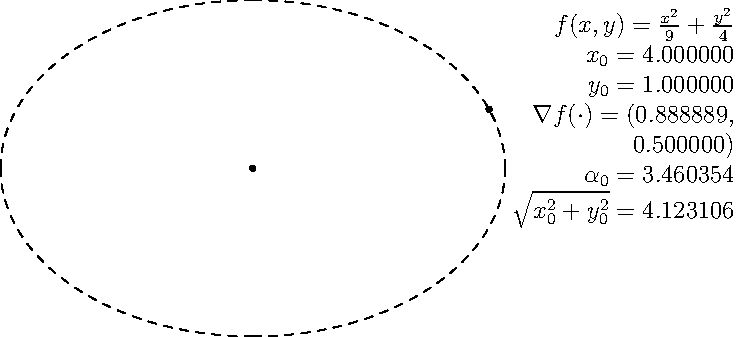
\includegraphics[width=\textwidth]{ellipse_grad2/ellipse_grad0}}%
\only<2-2>{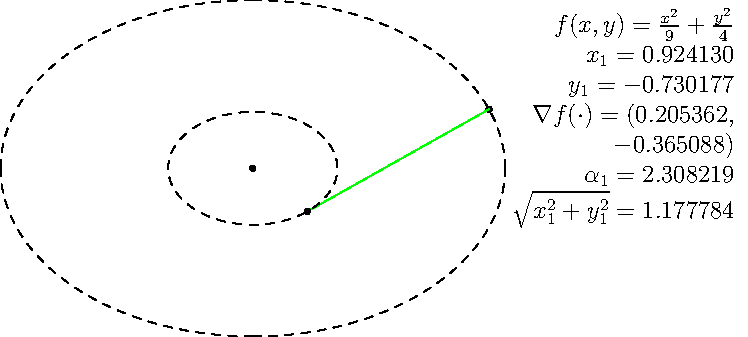
\includegraphics[width=\textwidth]{ellipse_grad2/ellipse_grad1}}%
\only<3-3>{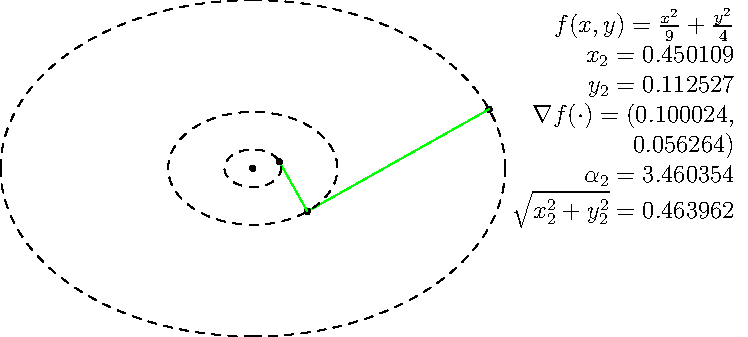
\includegraphics[width=\textwidth]{ellipse_grad2/ellipse_grad2}}%
\only<4-4>{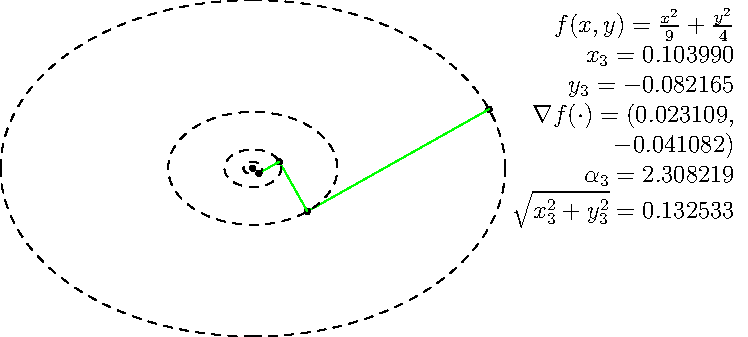
\includegraphics[width=\textwidth]{ellipse_grad2/ellipse_grad3}}%
\only<5-5>{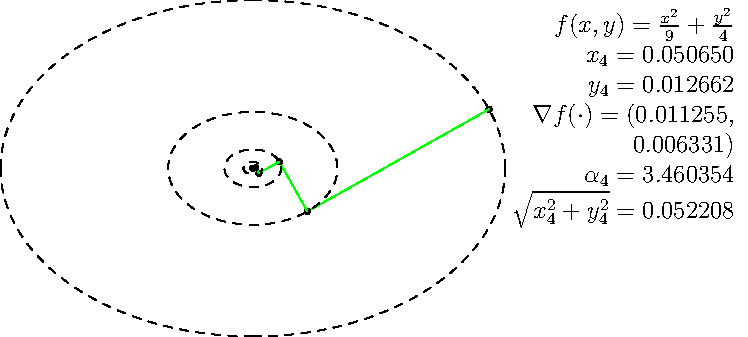
\includegraphics[width=\textwidth]{ellipse_grad2/ellipse_grad4}}%
\only<6-6>{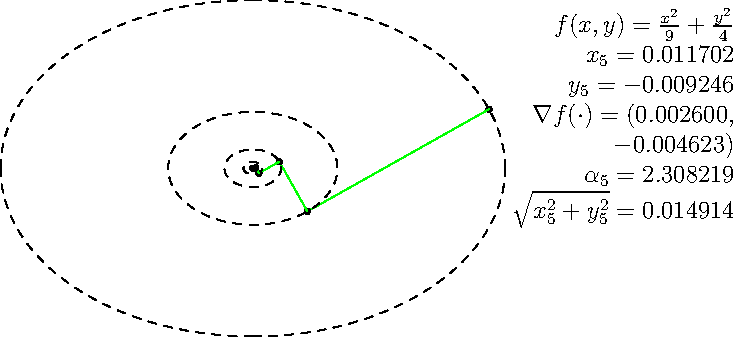
\includegraphics[width=\textwidth]{ellipse_grad2/ellipse_grad5}}%
\only<7-7>{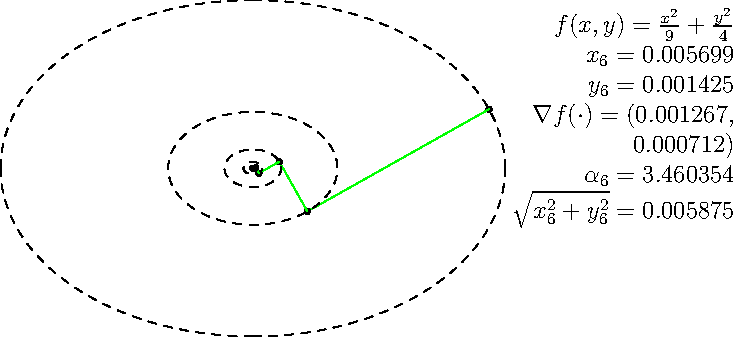
\includegraphics[width=\textwidth]{ellipse_grad2/ellipse_grad6}}%
\only<8-8>{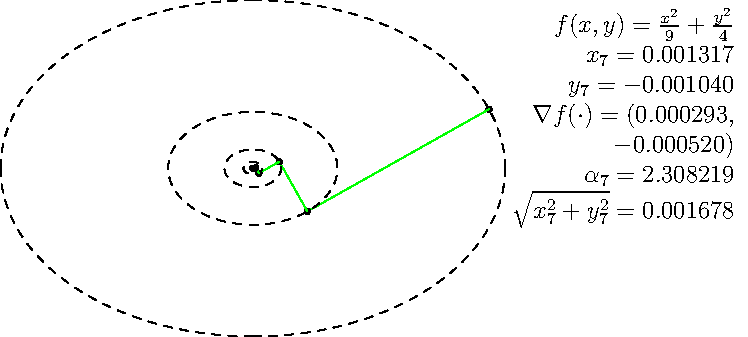
\includegraphics[width=\textwidth]{ellipse_grad2/ellipse_grad7}}%
\only<9-9>{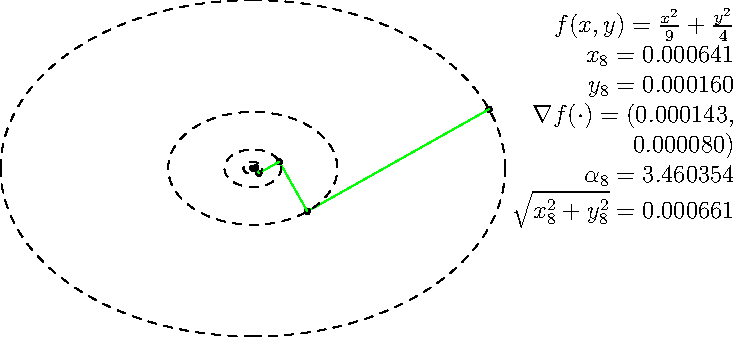
\includegraphics[width=\textwidth]{ellipse_grad2/ellipse_grad8}}%
\only<10-10>{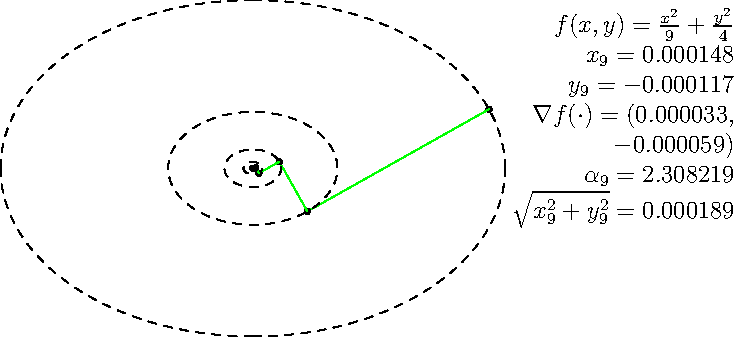
\includegraphics[width=\textwidth]{ellipse_grad2/ellipse_grad9}}%
\end{frame}

\begin{frame}{Пример: градиентный спуск для квадратичной функции}
\only<1-1>{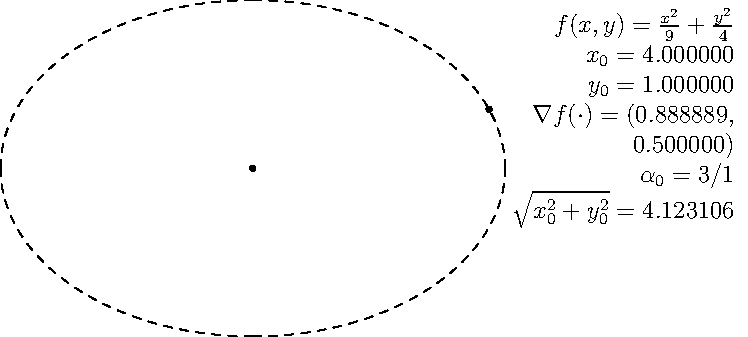
\includegraphics[width=\textwidth]{ellipse_grad3/ellipse_grad0}}%
\only<2-2>{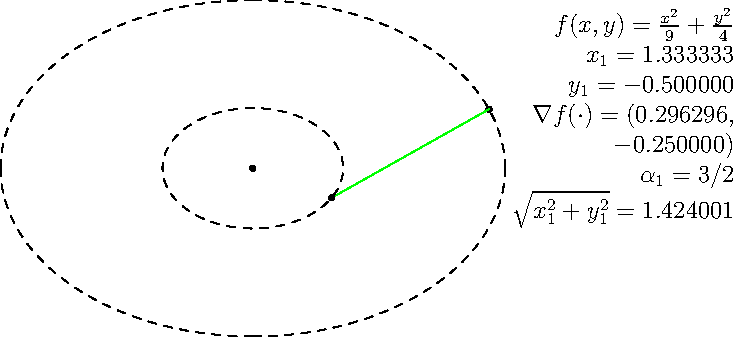
\includegraphics[width=\textwidth]{ellipse_grad3/ellipse_grad1}}%
\only<3-3>{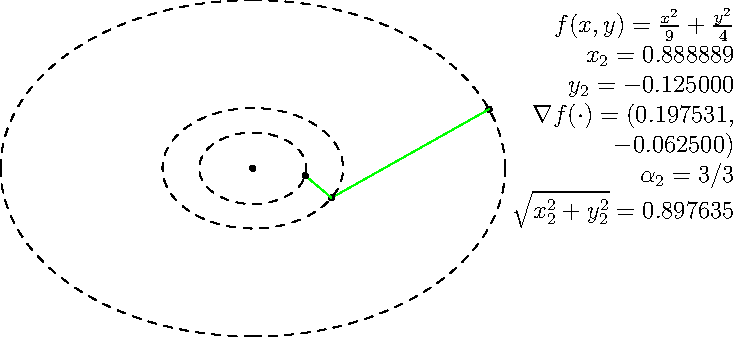
\includegraphics[width=\textwidth]{ellipse_grad3/ellipse_grad2}}%
\only<4-4>{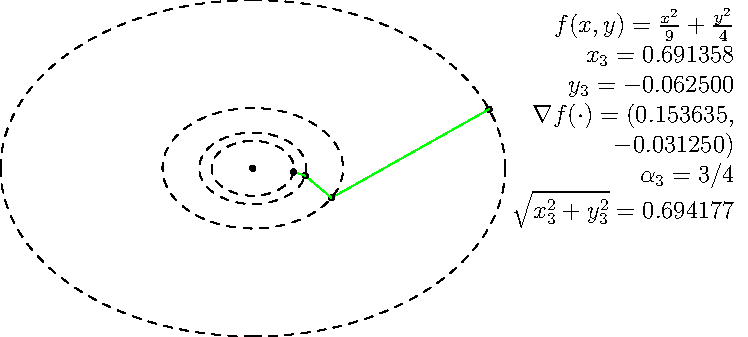
\includegraphics[width=\textwidth]{ellipse_grad3/ellipse_grad3}}%
\only<5-5>{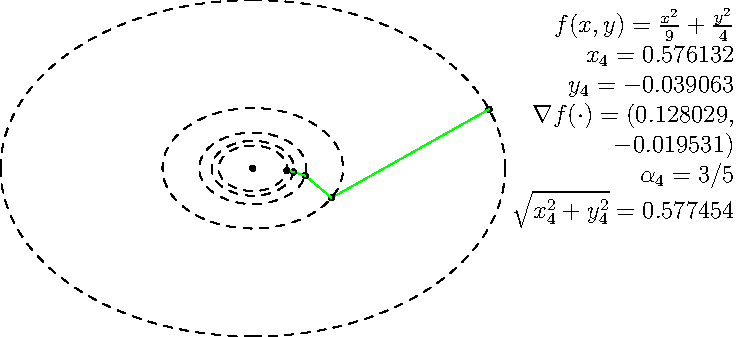
\includegraphics[width=\textwidth]{ellipse_grad3/ellipse_grad4}}%
\only<6-6>{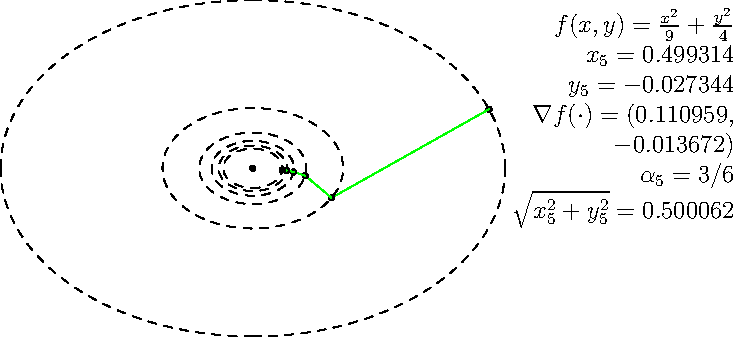
\includegraphics[width=\textwidth]{ellipse_grad3/ellipse_grad5}}%
\only<7-7>{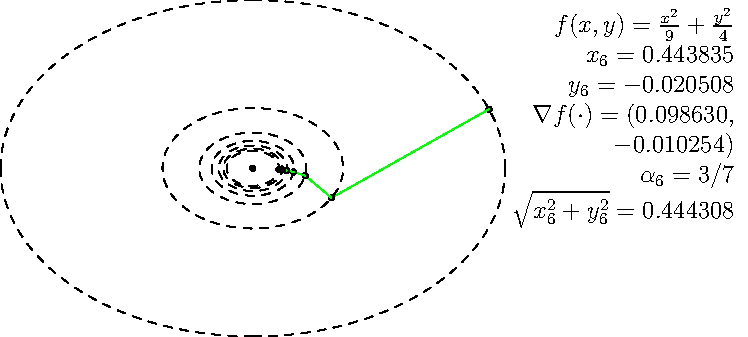
\includegraphics[width=\textwidth]{ellipse_grad3/ellipse_grad6}}%
\only<8-8>{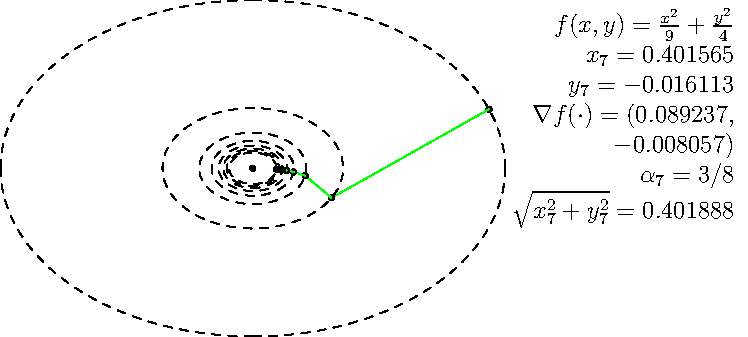
\includegraphics[width=\textwidth]{ellipse_grad3/ellipse_grad7}}%
\only<9-9>{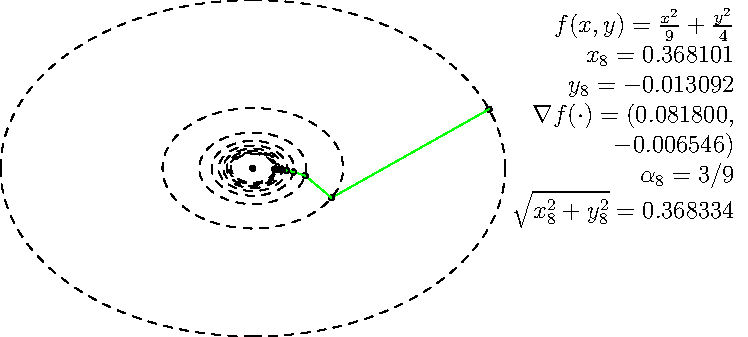
\includegraphics[width=\textwidth]{ellipse_grad3/ellipse_grad8}}%
\only<10-10>{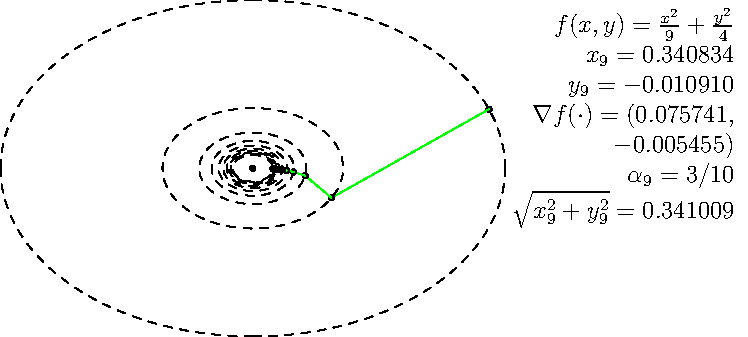
\includegraphics[width=\textwidth]{ellipse_grad3/ellipse_grad9}}%
\end{frame}

\begin{frame}{Предположения о минимизируемой функции}
В дальнейшем анализе будем полагать, что $f:\mathcal{D}\subset\mathbb{R}^n\rightarrow \mathbb{R}$ выпукла и дифференцируема на $\mathcal{D}$. Обозначим  
$$
S_f(x)=\{y\in\mathcal{D}~|~f(y)\leq f(x)\}.
$$ 
Также будут использоваться некоторые из следующих предположений:
\pause
\begin{itemize}[<+->]
\item Градиент $f$ непрерывен по Липшицу с константой $M$, т.е. 
$$||\nabla f(x)-\nabla f(y)||\leq M||x-y||~\forall x,y\in S_f(x_0).$$
\item $f$ -- сильно выпуклая функция с параметром $m$ на $S_f(x_0)$, т.е. $~\forall x,y\in S_f(x_0)$ 
$$
(\nabla f(y)-\nabla f(x))^T(y-x)\geq m||y-x||^2
$$
\end{itemize}
\pause
\textit{Замечание}. $S_f(x)$ -- выпуклое множество, если $f$ выпукла, более того $S_f(x)$ всегда ограничено, если $f$ сильно выпукла.
\end{frame}

\begin{frame}{Сходимость градиентного спуска}
\begin{theorem_ru}[Постоянный шаг]
Пусть $f$ выпукла и дифференцируема на $\mathcal{D}$, градиент $f$ липшицев с константой $M>0$ на $S_f(x_0)$, $f$ ограничена снизу,
существует хотя бы одна точка минимума $x^*$, $\alpha_k=\alpha\in [0, 1/M]$,
тогда для последовательности $x_k$, генерируемой по правилу \eqref{gradient_descent}  $f(x_k)$ убывает и, более того
$$
f(x_k)-f(x^*)\leq \frac{1}{2\alpha k}||x_0-x^*||^2.
$$
\end{theorem_ru}
\end{frame}


\begin{frame}{Сходимость градиентного спуска (постоянный шаг)}
\textbf{Док-во.} Используя непрерывность по Липшицу и $x_{k+1}-x_k=-\alpha \nabla f(x_k)$
\begin{align*}
f(x_{k+1})-f(x_k)&\leq \nabla f(x_k)^T(x_{k+1}-x_k)+\frac{M}{2}||x_{k+1}-x_k||^2\\
&=-\alpha\left(1-\frac{\alpha M}{2}\right)||\nabla f(x_k)||^2
\end{align*}
\pause
Таким образом $f(x_k)$ убывает в силу $0<\alpha<2/M$, что гарантирует $x_k\in S_f(x_0)$. \pause С другой стороны
$$
f(x_k)-f(x^*)\geq f(x_k)-f(x_{k+1})\geq \alpha\left(1-\frac{\alpha M}{2}\right)||\nabla f(x_k)||^2.
$$
Так как это неравенство выполняется при любом $\alpha\in(0, 2/M)$ и любом $x_k$, то минимизируя по $\alpha$ (минимум при $\alpha=1/M$) получаем
\begin{equation}\label{funcgeqgrad}
f(x)-f(x^*)\geq \frac{1}{2M}||\nabla f(x)||^2
\end{equation}
\end{frame}


\begin{frame}{Сходимость градиентного спуска (постоянный шаг)}
Вернемся на шаг назад, при условии $\alpha\leq 1/M$ выполняется $-\alpha+M\alpha^2/2\leq -\alpha/2$, получаем
\begin{align*}
f(x_{i+1}) & \leq f(x_i)-\alpha\left(1-\frac{\alpha M}{2}\right)||\nabla f(x_i)||^2 \\
& \leq f(x_i)-\frac{\alpha}{2}||\nabla f(x_i)||^2 \\
& \leq f(x^*)+\nabla f(x_i)^T(x_i-x^*)-\frac{\alpha}{2}||\nabla f(x_i)||^2 \\
& =f(x^*)+\frac{1}{2\alpha}\left(||x_i-x^*||^2-||x_i-x^*-\alpha \nabla f(x_i)||^2\right) \\
&=
f(x^*)+\frac{1}{2\alpha}\left(||x_i-x^*||^2-||x_{i+1}-x^*||^2\right).
\end{align*}
\pause
Суммируя по $i=0\ldots k-1$ получаем
\begin{align*}
\sum_{i=1}^k(f(x_i)-f(x^*)) & \leq \frac{1}{2\alpha}
\sum_{i=1}^k\left(||x_{i-1}-x^*||^2-||x_i-x^*||^2\right)\\
& =\frac{1}{2\alpha}\left(||x_0-x^*||^2-||x_k-x^*||^2\right)\leq \frac{1}{2\alpha}||x_0-x^*||^2. 
\end{align*}
\end{frame}

\begin{frame}{Сходимость градиентного спуска}
Так как $f(x_k)$ убывает, то
$$
f(x_k)-f(x^*)\leq \frac{1}{k}\sum_{i=1}^k(f(x_i)-f(x^*))\leq \frac{1}{2\alpha k}||x_0-x^*||^2.
$$
\pause
\textit{Замечание $1$.} Если использовать минимум по направлению, то величина $f(x_k)-f(x_{k+1})$ увеличиваются,
а значит все оценки сохраняются.\\
\end{frame}

\begin{frame}{Использование \textit{backtracking line search}}
\textit{Замечание $2$.} Если использовать аппроксимированный минимум по направлению 
с параметрами $\gamma\in(0, 1/2), \beta\in(0,1)$, то учитывая $-\alpha+M\alpha^2/2\leq -\alpha/2$ при $0\leq \alpha\leq 1/M$ 
\begin{align*}
f(x_k-\alpha\nabla f(x_k))&\leq f(x_k)-\alpha\left(1-\frac{\alpha M}{2}\right)||\nabla f(x_k)||^2\\
&\leq f(x_k)-\frac{\alpha}{2}||\nabla f(x_k)||^2
\end{align*}
получаем, что условие выхода в \textit{backtracking line search} выполняется для любого $\alpha\in [0, 1/M]$. Так как
на каждом шаге $\alpha$ увеличивается в $\beta$ раз, то \textit{backtracking line search} выдаёт либо $1$, либо
виличину $\alpha_k\geq \beta/M$, что дает
\begin{align*}
f(x_{i+1}) & \leq f(x_i)-\frac{\alpha_k}{2}||\nabla f(x_i)||^2 \\
& \leq f(x^*)+\nabla f(x_i)^T(x_i-x^*)-\frac{\alpha_k}{2}||\nabla f(x_i)||^2 \\
& =f(x^*)+\frac{1}{2\alpha_k}\left(||x_i-x^*||^2-||x_i-x^*-\alpha_k \nabla f(x_i)||^2\right) \\
&\leq 
f(x^*)+\frac{1}{2\min\{1, \beta/M\}}\left(||x_i-x^*||^2-||x_{i+1}-x^*||^2\right).
\end{align*}

\end{frame}

\begin{frame}{Использование \textit{backtracking line search}}
Суммируя по итерациям выводим схожый результат, отличающийся на константу $\alpha\rightarrow \min\{1, \beta/M\}$:
$$
f(x_k)-f(x^*)\leq \frac{1}{k}\sum_{i=1}^k(f(x_i)-f(x^*))\leq \frac{1}{2\min\{1, \beta/M\} k}||x_0-x^*||^2.
$$
\end{frame}

\begin{frame}{Сходимость градиентного спуска ($f(x_k)\rightarrow f(x^*)$)}
\begin{theorem_ru}[Постоянный шаг, сильная выпуклость] Пусть $f$ дифференцируема на $\mathcal{D}$, $\alpha_k\equiv \alpha\in (0, 2/M)$, $f$ сильно выпукла с константой $m>0$ на $S_f(x_0)$, градиент $f$ липшицев с константой $M\geq m$ на $S_f(x_0)$, тогда для последовательности $x_k$, генерируемой по правилу \eqref{gradient_descent},
$x_k$ cходится к единственной точке минимума $x^*$ $f$ на $\mathcal{D}$, $f(x_k)$ убывает и сходится к $f(x^*)$, более того для $q=1-2m\alpha+mM\alpha^2$
$$
f(x_k)-f(x^*)\leq q^k(f(x_0)-f(x^*)).
$$
\end{theorem_ru}
\end{frame}

\begin{frame}{Сходимость градиентного спуска ($f(x_k)\rightarrow f(x^*)$)}
\textbf{Док-во.} Из сильной выпуклости
$$
f(y)\geq f(x)+\nabla f(x)^T(y-x)+\frac{m}{2}||y-x||^2.
$$
Минимизирую правую часть по $y$ (минимум при $y=x-(1/m)\nabla f(x)$) получаем
$$
f(y)\geq f(x)-\frac{1}{2m}||\nabla f(x)||^2.
$$
В частности
\begin{equation}\label{funcleqgrad}
f(x)-f(x^*)\leq \frac{1}{2m}||\nabla f(x)||^2
\end{equation}
\pause
Наконец, вновь воспользовавшись сильной выпуклостью
$$
0\geq f(x^*)- f(x)\geq\nabla f(x)^T(x^*-x)+\frac{m}{2}||x-x^*||^2\geq
$$
$$
-||\nabla f(x)||\cdot||x^*-x||+\frac{m}{2}||x-x^*||^2,
$$
а значит
\begin{equation}\label{estleqgrad}
||x-x^*||\leq \frac{2}{m}||\nabla f(x)||.
\end{equation}
\end{frame}

\begin{frame}{Сходимость градиентного спуска ($f(x_k)\rightarrow f(x^*)$)}
Далее, так как $f(x_k)$ убывает, а $f$ ограничена снизу, то $f(x_k)$ сходится, более того
$$
f(x_0)-f(x^*)\geq \sum_{k=0}^\infty f(x_k)-f(x_{k+1})\geq \alpha\left(1-\frac{\alpha M}{2}\right)\sum_{k=0}^\infty||\nabla f(x_k)||^2.
$$
\pause
Таким образом ряд $\sum_{k=0}^\infty||\nabla f(x_k)||^2$ сходится $\Rightarrow$ $||\nabla f(x_k)||\rightarrow 0$, в силу \eqref{estleqgrad} $x_k\rightarrow x^*$ и, следовательно $f(x_k)\rightarrow f(x^*)$. \\
\pause
\vspace{1em}
Далее, оценим скорость сходимости: вернемся к неравенству
$$
f(x_{k+1})\leq f(x_k)-\alpha\left(1-\frac{\alpha M}{2}\right)||\nabla f(x_k)||^2.
$$
Вычитая из обоих частей $f(x^*)$ и используя \eqref{funcleqgrad} получаем
$$
f(x_{k+1})-f(x^*)\leq f(x_k)-f(x^*)-\alpha\left(1-\frac{\alpha M}{2}\right)2m(f(x_k)-f(x^*))
$$
\end{frame}

\begin{frame}{Сходимость градиентного спуска ($f(x_k)\rightarrow f(x^*)$)}
Таким образом
$$
f(x_{k})-f(x^*)\leq q(f(x_{k-1})-f(x^*))\leq q^k(f(x_0)-f(x^*)).~~\blacksquare
$$
\pause
\textit{Замечание 1.} Используя \eqref{funcgeqgrad} и \eqref{estleqgrad} можно получить 
$$
||x_k-x^*||^2\leq \frac{8M}{m^2}q^k(f(x_0)-f(x^*)).
$$
\pause
\textit{Замечание 2.} При использовании \textit{backtracking line search} с параметрами $\gamma, \beta$ все выкладки
сохраняются при $q=1-\min\{2m\gamma, 2\beta\gamma m/M\}$. 
\end{frame}

\begin{frame}{Сходимость градиентного спуска ($x_k\rightarrow x^*$)}
\begin{lemma_ru}[О $m$-сильно выпуклой $M$-гладкой функции]
Пусть $f:\mathcal{D}\rightarrow \mathbb{R}$ -- сильно выпуклая c параметром $m$ функция, $\nabla f$ удовлетворяет условию
Липшица с параметром $M$, т.~е.
$$
m||y-x||^2\leq (\nabla f(y)-\nabla f(x))^T(y-x)\leq M||y-x||^2,
$$
тогда для $f$ выполняется
$$
(\nabla f(y)-\nabla f(x))^T(y-x)\geq \frac{mM}{m+M}||y-x||^2+\frac{1}{m+M}||\nabla f(y)-\nabla f(x)||^2
$$
\end{lemma_ru}
\pause
\textbf{Док-во.} Рассмотрим функцию $g(x)=f(x)-\frac{m}{2}||x||^2$. Заметим, что $\nabla g(x)=\nabla f(x)-mx$ и
$$
(\nabla g(y)-\nabla g(x))^T(y-x)=(\nabla f(y)-\nabla f(x))^T(y-x)-m||y-x||^2,
$$
то есть $g$ -- выпуклая функция, $\nabla g$ удовлетворяет условию Липшица с константой $M-m$.
\end{frame}

\begin{frame}{Сходимость градиентного спуска ($x_k\rightarrow x^*$)}
Далее, пусть для некоторого $x$ $\phi(y)=g(y)-\nabla g(x)^Ty$. Заметим, что $\nabla \phi(y)=\nabla g(y)-\nabla g(x)$, таким
образом $\phi$ тоже выпукла и $\nabla \phi$ удовлетворяет условию Липшица с константов $M-m$.\\
\pause
\vspace{1em}
Точка $x$ минимизирует $\phi$ в силу выпуклости $\phi$ и $\nabla \phi(x)=0$, используя \eqref{funcgeqgrad}
$$
\phi(x)\leq \phi(y)-\frac{1}{2(M-m)}||\nabla \phi(y)||^2
$$
что имеет следующий вид в терминах $g$
$$
g(y)\geq g(x)+\nabla g(x)^T(y-x)+\frac{1}{2(M-m)}||\nabla g(y)-\nabla g(x)||^2
$$
\pause
складывая это неравенство с самим собой с переставленными $x\leftrightarrow y$ получаем
$$
(\nabla g(y)-\nabla g(x))^T(y-x)\geq \frac{1}{M-m}||\nabla g(y)-\nabla g(x)||^2
$$
\end{frame}

\begin{frame}{Сходимость градиентного спуска ($x_k\rightarrow x^*$)}
Наконец, выражая $g$ через $f$ получаем
\begin{align*}
(\nabla g(y)-\nabla g(x))^T(y-x)&=(\nabla f(y)-\nabla f(x))^T(y-x)-m||y-x||^2\\
||\nabla g(y)-\nabla g(x)||^2&=||\nabla f(y)-\nabla f(x)||^2-2m(\nabla f(y)-\nabla f(x))^T(y-x)\\
&~~~+m^2||y-x||^2,
\end{align*}
\pause
что дает
\begin{align*}
(\nabla f(y)-\nabla f(x))^T(y-x)&\geq m||y-x||^2+\frac{1}{M-m}(||\nabla f(y)-\nabla f(x)||^2\\
&~~~-2m(\nabla f(y)-\nabla f(x))^T(y-x)+m^2||y-x||^2)\\
\end{align*}
\pause
\begin{align*}
(\nabla f(y)-\nabla f(x))^T(y-x)&\geq \frac{1}{m+M}(Mm||y-x||^2+||\nabla f(y)-\nabla f(x)||^2)~~\blacksquare
\end{align*}
\end{frame}

\begin{frame}{Сходимость градиентного спуска ($x_k\rightarrow x^*$)}
\begin{theorem_ru}
Пусть $f$ дифференцируема на $\mathcal{D}$, $\alpha_k\equiv \alpha\in (0, 2/(M+m))$, $f$ сильно выпукла с константой $m>0$ на 
$\bar{B}(x^*, ||x_0-x^*||)$, градиент $f$ липшицев с константой $M\geq m$ на $\bar{B}(x^*, ||x_0-x^*||)$, тогда для последовательности $x_k$, генерируемой по правилу \eqref{gradient_descent},
$x_k$ cходится к единственной точке минимума $x^*$ $f$ на $\mathcal{D}$, более того для 
$$
||x_k-x^*||^2\leq \left(1-\frac{2\alpha mM}{M+m}\right)^k||x_0-x^*||^2
$$
\end{theorem_ru}
\pause
\textbf{Док-во.} Используя доказанную лемму
\begin{align*}
||x_{k+1}-x^*||^2&=||x_k-x^*||^2-2\alpha\nabla f(x_k)(x_k-x^*)+\alpha^2||\nabla f(x_k)||^2\\
&\leq \left(1-\frac{2\alpha mM}{M+m}\right)||x_k-x^*||^2+\alpha\left(\alpha-\frac{2}{m+M}\right)||\nabla f(x_k)||^2\\
&\leq \left(1-\frac{2\alpha mM}{M+m}\right)||x_k-x^*||^2
\end{align*}
\end{frame}

\begin{frame}{Оптимальность $\alpha=2/(m+M)$}
\textit{Замечание}. При $\alpha=2/(m+M)$ параметр сходимости становится
$$
1-\frac{2\alpha mM}{M+m}=1-\frac{4 mM}{(M+m)^2}=\left(\frac{M-m}{M+m}\right)^2
$$
\pause
Такой выбор $\alpha$ оптимален при условии, что $m, M$ -- точные оценки: пусть $f(x)=\frac{1}{2}x^TAx-b^Tx$, $A=A^T$, тогда 
последовательность \eqref{gradient_descent} принимает вид
$$
x_{k+1}=(I-\alpha A)x_k+\alpha b.
$$
\pause
Если  $Ax^*=b$, $m, M>0$ -- минимальное и максимальное собственные числа $A$, то
$$
||x_{k+1}-x^*||=||(I-\alpha A)(x_k-x^*)||\leq \max\{|1-\alpha M|, |1-\alpha m|\} ||x_k-x^*||,
$$
при этом
$$
 \min_\alpha\max\{|1-\alpha M|, |1-\alpha m|\}=\frac{M-m}{M+m},
$$
минимум достигается при $\alpha=2/(m+M)$.


\end{frame}

\begin{frame}{Ссылки на литературу}
\href{http://premolab.ru/pub_files/pub5/MnexoB89z7.pdf}{\textit{Нестеров Ю. Е.} Методы выпуклой оптимизации} // парагафы 1.2.3 и 2.1.5 \\
\vspace{1em}
\href{https://web.stanford.edu/~boyd/cvxbook/bv_cvxbook.pdf}{\textit{Boyd S., Vandenberghe L.} Convex optimization} // парагаф 9.3\\
\vspace{1em}
\href{http://lab7.ipu.ru/files/polyak/polyak-optimizationintro.pdf}{\textit{Поляк Б. Т.} Введение в оптимизацию} // парагаф 1.4\\
\vspace{1em}
\href{http://www.seas.ucla.edu/~vandenbe/236C/lectures/gradient.pdf}{\textit{Vandenberghe L.} Лекция по градиентному спуску} 

\end{frame}

\end{document}